%%%%%%%% ICML 2022 EXAMPLE LATEX SUBMISSION FILE %%%%%%%%%%%%%%%%%
\documentclass[nohyperref]{article}

% Recommended, but optional, packages for figures and better typesetting:
\usepackage{microtype}
\usepackage{graphicx}
\usepackage{subfigure}
\usepackage{booktabs} % for professional tables
\usepackage[]{acronym}

% hyperref makes hyperlinks in the resulting PDF.
% If your build breaks (sometimes temporarily if a hyperlink spans a page)
% please comment out the following usepackage line and replace
% \usepackage{icml2022} with \usepackage[nohyperref]{icml2022} above.
\usepackage{hyperref}

% Attempt to make hyperref and algorithmic work together better:
\newcommand{\theHalgorithm}{\arabic{algorithm}}

% Use the following line for the initial blind version submitted for review:
\usepackage[accepted]{icml2022}

\hypersetup{ %
	pdftitle={Impact of Dimensionality Reduction over a KNN},
	pdfauthor={Valentin Rieu, Amgad Khalil},
	pdfsubject={Machine Learning},
	pdfkeywords={},
	pdfborder=0 0 0,
	pdfpagemode=UseNone,
	colorlinks=true,
	linkcolor=mydarkblue,
	citecolor=mydarkblue,
	filecolor=mydarkblue,
	urlcolor=mydarkblue,
}

% If accepted, instead use the following line for the camera-ready submission:
% \usepackage[accepted]{icml2022}

% For theorems and such
\usepackage{amsmath}
\usepackage{amssymb}
\usepackage{mathtools}
\usepackage{amsthm}

% if you use cleveref..
\usepackage[capitalize,noabbrev]{cleveref}

%%%%%%%%%%%%%%%%%%%%%%%%%%%%%%%%
% THEOREMS
%%%%%%%%%%%%%%%%%%%%%%%%%%%%%%%%
\theoremstyle{plain}
\newtheorem{theorem}{Theorem}[section]
\newtheorem{proposition}[theorem]{Proposition}
\newtheorem{lemma}[theorem]{Lemma}
\newtheorem{corollary}[theorem]{Corollary}
\theoremstyle{definition}
\newtheorem{definition}[theorem]{Definition}
\newtheorem{assumption}[theorem]{Assumption}
\theoremstyle{remark}
\newtheorem{remark}[theorem]{Remark}

% Todonotes is useful during development; simply uncomment the next line
%    and comment out the line below the next line to turn off comments
%\usepackage[disable,textsize=tiny]{todonotes}
\usepackage[textsize=tiny]{todonotes}



\icmltitlerunning{Analysis of the Impact of Dimensionality Reduction over a KNN}
\begin{document}

	\twocolumn[
\icmltitle{Analysis of the Impact of Dimensionality Reduction over a K-Nearest Neighbor}

% It is OKAY to include author information, even for blind
% submissions: the style file will automatically remove it for you
% unless you've provided the [accepted] option to the icml2022
% package.

% List of affiliations: The first argument should be a (short)
% identifier you will use later to specify author affiliations
% Academic affiliations should list Department, University, City, Region, Country
% Industry affiliations should list Company, City, Region, Country

% You can specify symbols, otherwise they are numbered in order.
% Ideally, you should not use this facility. Affiliations will be numbered
% in order of appearance and this is the preferred way.
\icmlsetsymbol{equal}{*}

\begin{icmlauthorlist}
	\icmlauthor{Valentin Rieu}{ujm}
	\icmlauthor{Amgad Khalil}{ujm}
\end{icmlauthorlist}

\icmlaffiliation{ujm}{University Jean Monnet, Saint-Etienne, France}

\icmlcorrespondingauthor{Valentin Rieu}{valentin.rieu@etu.univ-st-etienne.fr}
\icmlcorrespondingauthor{Amgad Khalil}{amgad.khalil@etu.univ-st-etienne.fr}


% You may provide any keywords that you
% find helpful for describing your paper; these are used to populate
% the "keywords" metadata in the PDF but will not be shown in the document
\icmlkeywords{Machine Learning, KNN}

\vskip 0.3in
]

% this must go after the closing bracket ] following \twocolumn[ ...

% This command actually creates the footnote in the first column
% listing the affiliations and the copyright notice.
% The command takes one argument, which is text to display at the start of the footnote.
% The \icmlEqualContribution command is standard text for equal contribution.
% Remove it (just {}) if you do not need this facility.

%\printAffiliationsAndNotice{}  % leave blank if no need to mention equal contribution
\printAffiliationsAndNotice{} % otherwise use the standard text.


	\begin{abstract}
		In this article, we describe two Dimensionality Reduction methods used on a dataset in order to increase the accuracy of K-Nearest Neighbor algorithms.\\
		The utilization of Dimensionality Reduction methods such as Principal Component Analysis and Linear Discriminant Analysis help reduce the risks of overfitting in high dimensional datasets, and increase accuracies.
	\end{abstract}
	
	\section{Introduction}
	In classification problems, we may encounter phenomena that limits the accuracy of the classification, and may involve risks of overfitting during training time.\\
	One of those phenomena is the \textit{Curse of Dimensionality}, that can be defined as follows:
	\begin{quote}
		As the number of Features (or Dimensions) grows, the amount of Data we need to generalize accurately grows Exponentially.
	\end{quote}
	K-Nearest Neighbor (KNN) algorithms are strongly affected by the \textit{Curse of Dimensionality}, even with as low as 20 dimensions, because the computation of the distances between points become more expensive, and as the distance between points grows, the concept of neighbors becomes weaker \cite{Beyer1998}.\\
	To solve this problem, we have two solutions:
	\begin{description}
		\item[Increase the size of the dataset:] This solution presents two issues:
		\begin{enumerate}
			\item The number of samples required to overcome the \textit{Curse of Dimensionality} increases exponentially fast,
			\item It is not always possible to increase the size of a dataset, especially in domains where available data is sparse.
		\end{enumerate}
		\item[Reduce the dimensionality of the dataset:] Dimensionality Reduction consists of finding key ''components'' that describes the attributes of a dataset while preserving the information of said features.
	\end{description}
	
	\section{Methodology} 
	In this article, since the first solution is not applicable in most scenarios, we will explore the second solution, using Principal Component Analysis (PCA) \cite{Jackson1991} and Linear Discriminant Analysis (LDA) \cite{balakrishnama1998linear}\\
	We will use the waveform dataset built by \citet{waveform}, containing 5000 samples distributed within 3 classes. Each sample is described by 21 attributes, all of which contain noise and overlaps between classes. The optimal Bayes Classifier has an accuracy of 86\%.\\
	We consider three experiments, \textsc{Control} \textsc{PCA}, \textsc{LDA}, which corresponds to the execution of, respectively, no modification, a PCA, and an LDA over the original dataset.\\
	We consider three copies of the dataset $S$:
	\begin{itemize}
		\item $S_c$ is the dataset for \textsc{Control},
		\item $S_{\text{PCA}}$ is the dataset for \textsc{PCA}
		\item $S_{\text{LDA}}$ is the dataset for \textsc{LDA} 
	\end{itemize}
	For each dataset $S_i$, we split the datasets in two datasets, $T^R_i$ as the training set, and $T^E_i$ as the test set, by a ratio of 4:1 (4000 samples in $T^R_i$, 1000 samples in $T^E_i$).\\
	$T^E_i$ will not be used to compute the PCA and the LDA, nor will it be used to tune the hyperparameter $k$ of the different experiments. \\
	Once performing the different experiments, we will compute the accuracy of the different models over the respective test sets, and compare the results.
	
	\section{Results}
	
	After performing \textsc{PCA} and \textsc{LDA}, we managed to reduce the number of dimensions to, respectively 19 and 18 without loosing too much information. As shown in \cref{k-tuning}, the different approaches perform differently with different values of $k$, and the two Dimensionality Reduction methods \textsc{PCA} and \textsc{LDA} will perform better than \textsc{Control} with most of those values. They also manage to get over the optimal Bayes classification rate, which is not possible for the \textsc{Control} experiment.
	\begin{figure}[ht]
		\vskip 0.2in
		\begin{center}
			\centerline{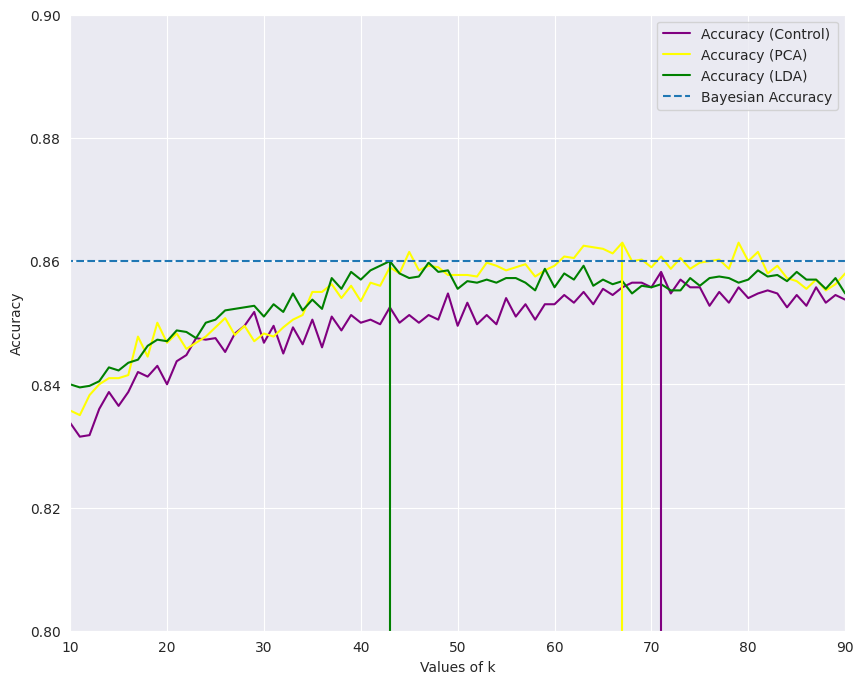
\includegraphics[width=\columnwidth]{img/k_tuning-pca-lda.png}}
			\caption{Accuracy of the models over the training set with different values of $k$. Bayesian Accuracy is depicted as a dashed line. Vertical lines indicate for which value of $k$ the models performed the best}
			\label{k-tuning}
		\end{center}
		\vskip -0.2in
	\end{figure}

	After training our models, we used the test sets to compute the accuracy of the different models over a set of unexplored data, on a KNN using their optimal hyperparameter $k$. As shown in \cref{results-table}, the \textsc{LDA} model performed the best and had the least amount of standard deviation on average. \textsc{Control} performed worse, however the difference between \textsc{Control} and \textsc{PCA} is not strong enough to conclude of an evident superiority.
	\begin{table}[ht]

		\begin{center}
			\begin{small}
				\begin{sc}
					\begin{tabular}{lcccc}
						\toprule
						Experiment & $k$ & Dimension & Accuracy         & $>$? \\
						\midrule
						Control    & 71  &    21     & 86.10 $\pm$ 2.36 & \\
						PCA		   & 67  &    19     & 86.20 $\pm$ 2.35 & $\approx$ \\
						LDA		   & 43  &    18     & 86.90 $\pm$ 1.88 & $\surd$ \\
						\bottomrule
					\end{tabular}
				\end{sc}
			\end{small}
		\end{center}
	\vskip -0.1in
	\caption{Dimensionality Reduction and Classification accuracies for the different experiments over the test set. Higher is better.}
	\label{results-table}
	\end{table}
	

	\begin{figure}[ht]
		\vskip 0.2in
		\begin{center}
			\centerline{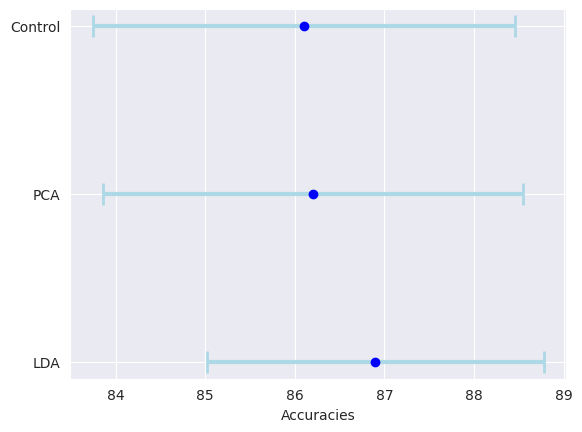
\includegraphics[width=\columnwidth]{img/lda-pca-error.png}}
			\caption{Accuracy bar of the different Approaches with $k$ tuned. Blue dot is the accuracy, bar represents the standard deviation}
			\label{results-error}
		\end{center}
		\vskip -0.2in
	\end{figure}

The similarity between \textsc{Control} and \textsc{PCA} is more evident when observing \cref{results-error} and the impact of their standard deviation.


\newpage
	\section{Conclusion}
	After analysis of our results, we can conclude on the effectiveness of Dimensionality Reduction on the given dataset. As the dimension of our data increases, Dimensionality Reduction becomes more and more essential especially for algorithms as impacted by dimensions as KNN is.\\
	LDA is the best algorithm in our context, as we managed to reduce the dimensions further while increasing the accuracy. Computation is also faster as $k$ has also been lowered in the process.\\
	Further analysis may include other Dimensionality Reduction methods such as t-SNE, \textit{kernel}-PCA, or
	UMAP, and the impact of those methods on imbalanced dataset.
	


\bibliography{main}
\bibliographystyle{icml2022}		
	
	%%%%%%%%%%%%%%%%%%%%%%%%%%%%%%%%%%%%%%%%%%%%%%%%%%%%%%%%%%%%%%%%%%%%%%%%%%%%%%%
	%%%%%%%%%%%%%%%%%%%%%%%%%%%%%%%%%%%%%%%%%%%%%%%%%%%%%%%%%%%%%%%%%%%%%%%%%%%%%%%
	% APPENDIX
	%%%%%%%%%%%%%%%%%%%%%%%%%%%%%%%%%%%%%%%%%%%%%%%%%%%%%%%%%%%%%%%%%%%%%%%%%%%%%%%
	%%%%%%%%%%%%%%%%%%%%%%%%%%%%%%%%%%%%%%%%%%%%%%%%%%%%%%%%%%%%%%%%%%%%%%%%%%%%%%%
	
	%%%%%%%%%%%%%%%%%%%%%%%%%%%%%%%%%%%%%%%%%%%%%%%%%%%%%%%%%%%%%%%%%%%%%%%%%%%%%%%
	%%%%%%%%%%%%%%%%%%%%%%%%%%%%%%%%%%%%%%%%%%%%%%%%%%%%%%%%%%%%%%%%%%%%%%%%%%%%%%%
	
	
\end{document}


% This document was modified from the file originally made available by
% Pat Langley and Andrea Danyluk for ICML-2K. This version was created
% by Iain Murray in 2018, and modified by Alexandre Bouchard in
% 2019 and 2021 and by Csaba Szepesvari, Gang Niu and Sivan Sabato in 2022. 
% Previous contributors include Dan Roy, Lise Getoor and Tobias
% Scheffer, which was slightly modified from the 2010 version by
% Thorsten Joachims & Johannes Fuernkranz, slightly modified from the
% 2009 version by Kiri Wagstaff and Sam Roweis's 2008 version, which is
% slightly modified from Prasad Tadepalli's 2007 version which is a
% lightly changed version of the previous year's version by Andrew
% Moore, which was in turn edited from those of Kristian Kersting and
% Codrina Lauth. Alex Smola contributed to the algorithmic style files.
